
\de{ĐỀ THI HỌC KỲ I NĂM HỌC 2022-2023}{THPT Phạm Phú Thứ}


%Cau 1
\begin{bt}%[0T2B1-2]%[Dự án đề kiểm tra HKII NH22-23- PHẠM VĂN LONG]%[PHẠM PHÚ THỨ]
	 Biểu diễn miền nghiệm của bất phương trình $x-y-2<0$ trên mặt phẳng tọa độ $Oxy$.
	 \loigiai{
	 \immini{Vẽ đường thẳng $(\Delta) \colon x-y-2=0$ qua hai điểm $(2;0)$ và $(0;-2)$.\\
	 Xét gốc tọa độ $O\left(0;0\right)$. Ta thấy $O \notin \Delta $ và $0-0-2<0$. Do đó miền nghiệm của bất phương trình là nửa mặt phẳng không kể bờ $\Delta$ và chứa gốc tọa độ $O$ (miền không gạch chéo trên hình bên).}
	 {\begin{tikzpicture}[line join = round, line cap = round,>=stealth,font=\footnotesize,scale=1]
	 	\def\xmin{-1.5} \def\xmax{4}
	 	\def\ymin{-4.5} \def\ymax{2}
	 	\fill[pattern=north west lines] (\xmin,\ymin)--(\xmin,-3.5)--(4,\ymax)--(4,\ymin);
	 	\foreach \x in {1,2,3,3} \draw (\x,2pt)--(\x,-2pt) node [below] {$\x$};
	 	\draw[-stealth] (\xmin,0)--(\xmax,0)node[below]{$x$};
	 	\foreach \y in {-1,-2,-3,-4} \draw (2pt,\y)--(-2pt,\y) node [left] {$\y$};
	 	\draw[-stealth] (0,\ymin)--(0,\ymax)node[right]{$y$};
	 	\filldraw (0,0)node[below left]{$O$} circle (1.2pt);
	 	\clip (\xmin,\ymin) rectangle (\xmax,\ymax);	 	
	 	\draw[samples=100,domain=\xmin:\xmax,smooth] plot (\x, {(\x)-2});
	 \end{tikzpicture}}
 }	 
\end{bt} 
%Cau 2
\begin{bt}%[0T3B1-2]%[Dự án đề kiểm tra HKII NH22-23- PHẠM VĂN LONG]%[PHẠM PHÚ THỨ]
Tìm tập xác định của các hàm số sau
\begin{enumerate}
	\item $y=\dfrac{3 x+1}{x^2-10 x+9}$;
	\item $y=\dfrac{2}{x-7}-\sqrt{5 x+15}$. 	
\end{enumerate}
\loigiai{
\begin{enumerate}
	\item Điều kiện $x^2-10 x+9\ne 0\Leftrightarrow \heva{&x\ne 1\\&x\ne 9.}$\\
	Vậy $D=\mathbb{R}\setminus\left\{1;9\right\}$.
	\item Điều kiện $\heva{&x-7 \ne 0\\&5x+15\ge 0}\Leftrightarrow \heva{&x\ne 7\\&x\ge -3.}$\\	
	Vậy $D=[-3;+\infty)\setminus\left\{7\right\}$.
\end{enumerate}
}
\dapso{ a) $D=\mathbb{R}\setminus\left\{1;9\right\}$; b) $D=[-3;+\infty)\setminus\left\{7\right\}$.}

\end{bt}
%Cau 3
\begin{bt}%[0T3B2-3]%[Dự án đề kiểm tra HKII NH22-23- PHẠM VĂN LONG]%[PHẠM PHÚ THỨ]
	Khảo sát sự biến thiên và vẽ đồ thị hàm số $y=x^2-6x+5$.\\
	\loigiai{
		\begin{itemize}
			\item Khảo sát sự biến thiên:\\
			Đỉnh $S$ có tọa độ $ x_S=-\dfrac{b}{2a}=-\dfrac{-6}{2\cdot 1}=3$; $ y_S=-4$.\\
			Vì hàm số bậc hai có $ a=1>0 $ nên ta có bảng biến thiên sau
			\begin{center}
				
\begin{tikzpicture}
					\tkzTabInit[espcl=2.5,lgt=1.5,nocadre=false]
					{$x$/1,$f(x)$/2.1}
					{$-\infty$,$3$,$+\infty$}
					\tkzTabVar{+/$+\infty$,-/$-4$,+/$+\infty$}
				\end{tikzpicture}
			\end{center}
			Hàm số đồng biến trên $ \left(3;+\infty\right) $, nghịch biến trên $ \left(-\infty;3\right) $.\\
			Hàm số đạt giá trị nhỏ nhất bằng $ -4$ khi $ x=3$.
			\item Vẽ đồ thị:
			\immini{
				Trong mặt phẳng tọa độ $ Oxy $, đồ thị hàm số bậc hai $ y=f(x)=x^2-6x+5$ là một parabol $ (P)\colon $
				\begin{itemize}
					\item Có đỉnh $ S $ với hoành độ $ x_S=3$, tung độ $ y_S=-4 $;
					\item Có trục đối xứng là đường thẳng $ x=3$ (đường thẳng này đi qua đỉnh $ S $ và song song với trục $ Oy $);
					\item Bề lõm quay lên vì $ a>0 $;
					\item Cắt trục tung tại điểm có tung độ bằng $5$, cắt trục hoành tại hai điểm có tọa độ $(1;0)$ và $(5;0)$.
				\end{itemize}
			}
			{
				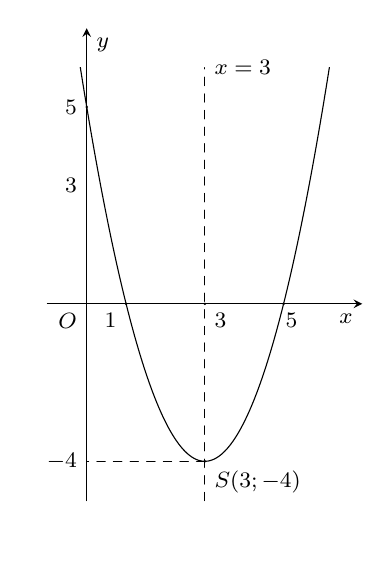
\begin{tikzpicture}[scale=0.5, font=\footnotesize,line join=round, line cap=round, >=stealth];
					\draw[->] (-1,0)--(7,0) node[below left ] {$x$};
					\draw[->] (0,-5)--(0,7) node[below right] {$y$};
					\draw (0,0) node [below left] {$O$} (1,0) node [below left] {$1$} (3,0) node [below right ] {$3$} (0,3) node [left] {$3$};
					\draw[dashed] (3,-4)node[below right]{$ S(3;-4) $}--(0,-4)node[left]{$-4 $} 
					(3,-5)--(3,6)node[right]{$ x=3 $}
					;
					\fill (1,0) circle (1pt) (5,0) circle (1pt); 
					\fill (3,0) circle (1pt); \fill (3,-4) circle (1pt);  \fill (0,5) circle (1pt);
					\foreach \x in {}
					\draw[thin] (\x,1pt)--(\x,-1pt) node [below] {$\x$};
					\foreach \y in {}
					\draw[thin] (1pt,\y)--(-1pt,\y) node [left] {$\y$};
					\begin{scope}
						\clip (-1.5,-6) rectangle (7,6);
						\draw[samples=200,domain=-1:7,smooth,variable=\x] plot (\x,{1*(\x)^2-6*(\x)+5});
					\end{scope}
				\draw (5.2,0) node [below] {$5$} (0,5) node [left] {$5$};
			\end{tikzpicture}	}
		\end{itemize}}
\end{bt} 
%Cau 4
\begin{bt}%[0T3B2-2]%[Dự án đề kiểm tra HKII NH22-23- PHẠM VĂN LONG]%[PHẠM PHÚ THỨ]
	Xác định parabol $(P): y=ax^2+bx-3$ biết $(P)$ có đỉnh $I(-1;-4)$.\\
	\loigiai{
		Parabol $(P): y=ax^2+bx-3$ có đỉnh $I(-1;-4)$ nên ta có:\\
		$$\heva{&-\dfrac{b}{2a}=-1\\&-4=a-b-3}\Leftrightarrow \heva{&2a-b=0\\&a-b=-1}\Leftrightarrow \heva{&a=1\\&b=2.}$$
		Vậy $(P): y=x^2+2x-3$
	}
\end{bt}
%Cau 5
\begin{bt}%[0T6B3-3]%[Dự án đề kiểm tra HKII NH22-23- PHẠM VĂN LONG]%[PHẠM PHÚ THỨ]
	Hãy tìm số trung bình và mốt của mẫu số liệu sau
	\begin{center}
		\begin{tabular}{|c|c|c|c|c|c|}
			\hline Giá trị & 6 & 7 & 8 & 9 & 10 \\
			\hline Tần số & 5 & 8 & 4 & 2 & 1 \\
			\hline
		\end{tabular}
	\end{center}
\loigiai{
	\begin{itemize}
		\item Trung bình $X=\dfrac{6\cdot 5+7\cdot 8+8\cdot 4+9\cdot 2+10\cdot 1}{20}=7{,}3$.
		\item $M_0=7$.
	\end{itemize}
}

\end{bt} 

%Cau 6
\begin{bt}%[0T5B2-2]%[0T5B3-2] %[Dự án đề kiểm tra HKII NH22-23- NGUYỄN NGỌC DŨNG]%[PHẠM PHÚ THỨ]
\begin{enumerate}
\item Cho 6 điểm bất kì $A$, $B$, $C$, $H$, $K$, $I$. Chứng minh rằng $\overrightarrow{A B}-\overrightarrow{H C}-\overrightarrow{I K}=\overrightarrow{C I}-\overrightarrow{H A}+\overrightarrow{K B}$.	
\item Cho tứ giác $A B C D$. Gọi $M$, $N$ lần lượt là trung điểm của $BC$ và $CD$. Chứng minh rằng $2(\overrightarrow{AB}+\overrightarrow{NA}+\overrightarrow{AM}+\overrightarrow{DA})=3 \overrightarrow{DB}$.	
\end{enumerate}
\loigiai{
\begin{enumerate}
\item Ta có
\allowdisplaybreaks 
\begin{eqnarray*}
\overrightarrow{A B}-\overrightarrow{H C}-\overrightarrow{I K}=\overrightarrow{C I}-\overrightarrow{H A}+\overrightarrow{K B} 
&\Leftrightarrow& \vec{AB}+\vec{BK}+\vec{CH}+\vec{HA}+\vec{KI}+\vec{IC}=\vec{0} \\
&\Leftrightarrow& \vec{AK}+\vec{CA}+\vec{KC}=\vec{0} \\
&\Leftrightarrow& \vec{CC}=\vec{0} \text{ (luôn đúng)}.	
\end{eqnarray*}
Vậy $\overrightarrow{A B}-\overrightarrow{H C}-\overrightarrow{I K}=\overrightarrow{C I}-\overrightarrow{H A}+\overrightarrow{K B}$.	
\item Ta có
\immini{
\allowdisplaybreaks 
\begin{eqnarray*}
&& 2(\overrightarrow{AB}+\overrightarrow{NA} +\overrightarrow{AM}+\overrightarrow{DA})=3 \overrightarrow{DB} \\
&\Leftrightarrow& 2(\vec{DA}+\vec{AB}+\vec{NA}+\vec{AM})=3\vec{DB} \\
&\Leftrightarrow& 2(\vec{DB}+\vec{NM})=3\vec{DB}	
\end{eqnarray*}
Do $M, N$ là trung điểm $BC$ và $CD$ nên $\vec{NM}=\dfrac{1}{2}\vec{DB}$.\\
Thay vào đẳng thức, ta được
\[2\left(\vec{DB}+\dfrac{1}{2}\vec{DB}\right)=3\vec{DB} \Leftrightarrow 3\vec{DB}=3\vec{DB}.\]
}
{
\begin{tikzpicture}[line join = round, line cap = round, >=stealth, font=\footnotesize, scale=0.4]
\tikzset{label style/.style={font=\footnotesize}}
\coordinate[label=below:$A$] (A) at (0,0);
\coordinate[label=above:$B$] (B) at (4,6);
\coordinate[label=above:$C$] (C) at (12,6);
\coordinate[label=below:$D$] (D) at (12,-2);
\coordinate[label=above:$M$] (M) at ($(B)!.5!(C)$);
\coordinate[label=right:$N$] (N) at ($(D)!.5!(C)$);
\draw (A)--(B)--(C)--(D)--(A) (M)--(N) (B)--(D);
\end{tikzpicture}
}
\end{enumerate}
}
\end{bt}
%Cau 7
\begin{bt}%[0T5B2-5]%[Dự án đề kiểm tra HKII NH22-23- NGUYỄN NGỌC DŨNG]%[PHẠM PHÚ THỨ]
Cho hình chữ nhật $A B C D$ có $A B=4 a$, $A D=3 a$. Tính độ dài vectơ $\left|2 \overrightarrow{A B}-\overrightarrow{A C}\right|$.\\
\dapso{$\left|2 \overrightarrow{A B}-\overrightarrow{A C}\right|=5a$  }
\loigiai{
\immini{
Ta có
\allowdisplaybreaks 
\begin{eqnarray*}
&&2 \overrightarrow{A B}-\overrightarrow{A C} = \vec{AB}+\vec{AB}-\vec{AC}=\vec{AB}+\vec{CB}=\vec{AB}+\vec{DA}=\vec{DB} \\
&\Rightarrow& \left|2 \overrightarrow{A B}-\overrightarrow{A C}\right| = \left|\vec{DB}\right|=DB=5a.	
\end{eqnarray*}
}{
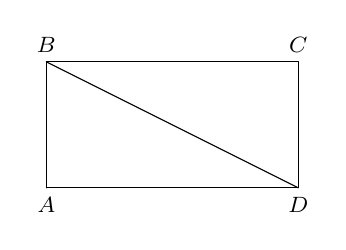
\begin{tikzpicture}[line join = round, line cap = round, >=stealth, font=\footnotesize, scale=0.8]
\tikzset{label style/.style={font=\footnotesize}}
\coordinate[label=below:$A$] (A) at (0,0);
\coordinate[label=above:$B$] (B) at (0,2);
\coordinate[label=above:$C$] (C) at (4,2);
\coordinate[label=below:$D$] (D) at (4,0);
\draw (A)--(B)--(C)--(D)--(A);
\draw (B)--(D);
\end{tikzpicture}
}
}
\end{bt} 
%Cau 8
\begin{bt}%[0T5B4-1]%[Dự án đề kiểm tra HKII NH22-23- NGUYỄN NGỌC DŨNG]%[PHẠM PHÚ THỨ]
Cho tam giác $A B C$ vuông tại $B$ có $B A=6$, $B C=8$. Gọi $M$ là điểm thưộc cạnh $A C$ sao cho $M A=2 M C$. Tính tích vô hướng $\overrightarrow{M A} \cdot \overrightarrow{M C}$.\\
\dapso{ $\overrightarrow{M A} \cdot \overrightarrow{M C}=\dfrac{-200}{9}$}
\loigiai{
Ta có $AC=\sqrt{AB^2+BC^2}=10$.\\
Mặt khác
$\heva{&MA=2MC \\ &MA+MC=AC} \Leftrightarrow \heva{&MA-2MC=0\\&MA+MC=10} \Leftrightarrow \heva{&MA=\dfrac{20}{3} \\ &MC =\dfrac{10}{3}}$.\\
Vậy $\vec{MA} \cdot \vec{MC}=\left|\vec{MA}
\right| \cdot \left| \vec{MC} \right| \cdot \cos \left(\vec{MA},\vec{MC}\right) = \dfrac{20}{3} \cdot \dfrac{10}{3} \cdot \cos 180^\circ = \dfrac{-200}{9}$.
}
\end{bt}
%Cau 9
\begin{bt}%[0T3K2-5]%[Dự án đề kiểm tra HKII NH22-23- NGUYỄN NGỌC DŨNG]%[PHẠM PHÚ THỨ]
Một rạp chiếu phim có sức chứa $1000$ người. Với giá vé là $40$ nghìn đồng, trung bình sẽ có khoảng $300$ người đến rạp xem phim mỗi ngày. Để tăng số lượng vé bán ra, rạp chiếu phim đã khảo sát thị trường và thấy rằng nếu giá vé cứ giảm $10$ nghìn đồng thì sẽ có thêm $100$ người đến rạp mỗi ngày. Tìm công thức của hàm số $R(x)$ mô tả doanh thu từ tiền bán vé mỗi ngày của rạp chiếu phim khi giá vé là $x$ nghìn đồng.\\
\dapso{$700x-10x^2$}
\loigiai{
Gọi $x$ (nghìn đồng) là giá vé ($x \in \{10, 20, 30, 40\}$).\\
Số người đến rạp tăng thêm so với khi giá vé là $40$ nghìn đồng là 
$$(40-x)\cdot \dfrac{100}{10} = (40-x)\cdot 10 \text{ (người)}.$$
Suy ra số người đến rạp là $300+(40-x)\cdot 10=700-10x$ (người).\\
Vậy doanh thu mỗi ngày khi giá vé là $x$ nghìn đồng là 
$$R(x)=(700-10x)\cdot x=700x-10x^2 \text{ (nghìn đồng)}.$$
}
\end{bt}